\chapter{Galaxy Vivisection}
\label{ch:galviv}

The preliminary investigation presented in Chapter \ref{ch:recov-mn} \citep{savorgnan2013} 
demonstrated the need for a new, systematic and homogeneous study 
aimed at obtaining more accurate galaxy decompositions 
and refining our knowledge about black hole mass scaling relations. 
In 2013, I visited A.~Marconi, E.~Sani, and L.~K.~Hunt (co-authors of the paper \citealt{sani2011}) 
in Arcetri (Florence) for a short collaboration, 
during which I was shown their 2D galaxy decomposition method using {\tt GALFIT3} \citep{peng2010}. 
This helped set the basis for the development of my own galaxy decomposition strategy. \\

Building on the catalog of \cite{grahamscott2013} 
with the addition of some new black hole mass measurements later published by \cite{rusli2013bhmassesDM}, 
I assembled my initial sample of 75 galaxies. 
For the imaging data, 
I chose to use \emph{Spitzer} archival observations at $3.6~\mu \rm m$ for three main reasons: 
(\emph{i}) the $3.6~\mu \rm m$ passband is currently the best proxy for the stellar mass 
(\citealt{sheth2010}, and references therein); 
(\emph{ii}) archival observations were publicly available for the majority of the galaxies in my initial sample; 
and (\emph{iii}) within a \emph{Spitzer} observation set of a galaxy, 
roughly half of the telescope pointings are dedicated to the imaging of the surrounding sky, 
ensuring a robust background determination during the data reduction process\footnote{These three points put together 
led me to prefer \emph{Spitzer} rather than \emph{HST} observations, 
albeit the lower spatial resolution. }. 
While for each galaxy \cite{sani2011} used only one set of \emph{Spitzer} astronomical observations, 
I downloaded all the publicly available observation sets and merged them into a single mosaic with higher signal-to-noise. 
I paid particular attention to (and invested a consistent amount of time into) the characterisation of the 
2D Point Spread Function (PSF), following the expert advice of C.~Peng. \\

Being aware of the importance of choosing the correct galaxy model 
in order to obtain reliable and meaningful structural parameters, 
I embraced the approach of \cite{laurikainen2005} 
and planned \emph{a priori} identification of the number and nature of the structural components in each galaxy. 
Given the lack of reference literature about advantages and disadvantages 
related to 1D and 2D decomposition techniques, 
I decided to experiment with both. \\ 

I wrote substantial software to perform 1D decomposition of surface brightness profiles. 
This code is written in {\tt Python} and is based on the Levenberg-Marquardt minimisation routine 
of the {\tt scipy.optimize} module. 
This software allows the user to build a galaxy model with any arbitrary number of analytical functions 
(S\'ersic, exponential, Gaussian, Ferrer, etc.). 
Because the code is written in an object-oriented fashion, 
it is particularly easy to implement any new analytical function into it. \\ 

For the 2D analysis, I experimented with the codes {\tt GALFIT3} \citep{peng2010} 
and {\tt Imfit} \citep{imfit}. 
After checking that both codes give consistent results, 
I preferred the more script-oriented {\tt Imfit} over {\tt GALFIT3}. \\ 

The NASA/IPAC Extragalactic Database (NED) has been an invaluable resource 
for the structural analysis of galaxies. 
NED lists all the literature references contained in the SAO/NASA Astrophysics Data System (ADS) 
which mentioned a particular galaxy. 
Thanks to this functionality, 
I was able to search for previous photometric and kinematic analyses, 
structural decompositions, information about the nuclear activity, 
presence of dust or peculiar features, 
and any other detail that could be useful to the analysis of my galaxies. \\

The remainder of this chapter comprises the published version of the paper 
``Supermassive Black Holes and Their Host Spheroids. I. Disassembling Galaxies'' 
by G.~A.~D.~Savorgnan \& A.~W.~Graham,  
as it appears in Volume 222 of the \emph{The Astrophysical Journal Supplement Series}. 


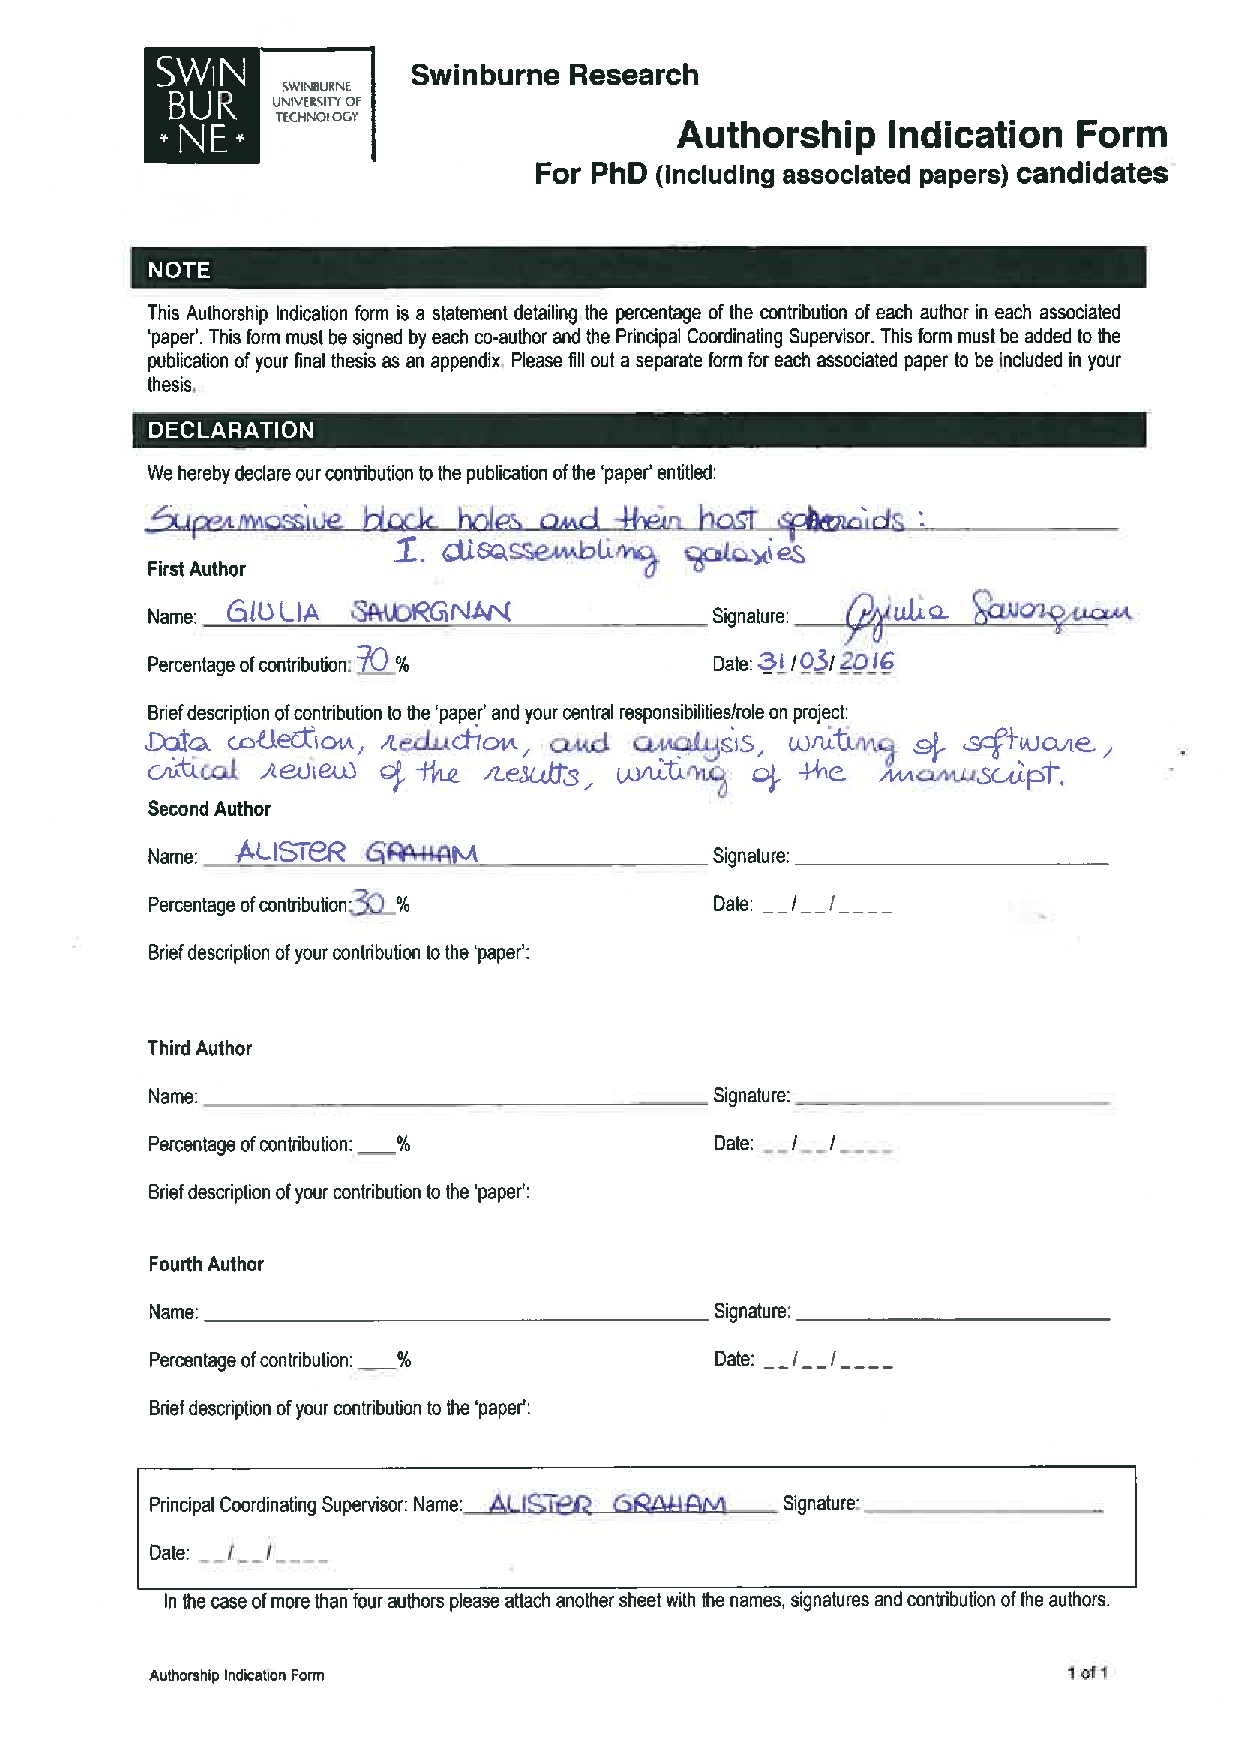
\includepdf[pages={1-58}]{ApJS2016.pdf}
